\documentclass[12pt]{article}
\usepackage{anyfontsize}
\usepackage[margin = 2cm]{geometry}
\usepackage{polski}
\usepackage[utf8]{inputenc}
\usepackage{tabto}
\usepackage{graphicx}
\usepackage{amsmath}
\usepackage{multicol}

% Dot post number of section
\usepackage{titlesec}
% Underline section, dot post number and span post dot
\titleformat{\section}
    {\Large \bfseries}
    {\thesection.}
    {0.5 cm}
    {}[\titlerule]
\titlelabel{\thetitle.\quad}


\usepackage{hyperref}
\hypersetup{
    colorlinks=true,
    linkcolor=black,
    filecolor=magenta,      
    urlcolor=cyan,
    pdfpagemode=FullScreen,
}

\usepackage{listings}


% \usepackage{csvsimple}
% \usepackage{pgfplots}

\usepackage[european, american currents, americanvoltages, RPvoltages]{circuitikz}
\usepackage{tikz}

\title{\underline{Systemy mikroprocesorowe}\\\textbf{Dokumentacja projektu}\\Azor - The czołg}
\author{Piotr Kowol, Łukasz Przystupa}
\date{\today}


\usepackage{titling}
\renewcommand\maketitlehooka{\null\mbox{}\vfill}
\renewcommand\maketitlehookd{\vfill\null}

% \pgfplotsset{compat=1.18}

% \usetikzlibrary{shapes.geometric}


\begin{document}
    \maketitle
    \begin{center}
        Opiekun: Jacek Ostrowski
    \end{center}
    \thispagestyle{empty}
    \newpage


    \section*{Streszczenie}
    \tab Kilka słów podsumowujących pracę. Do napisania na \textbf{koniec}
    \thispagestyle{empty}
    \newpage
    
    \tableofcontents
    \newpage
    \section*{Wstęp}
\phantomsection
\addcontentsline{toc}{section}{\protect\numberline{}Wstęp}
    \tab Też do napisania potem

    \section{Cel i założenia projektowe}
    \tab Powyższy projekt oparty jest o mikrokontroler z rodziny AVR: ATmega8A.
    Komunikując się z odpowiedniki sensorami jest w stanie zlokalizować się w przestrzeni,
    oraz stworzyć prostą mapę pomieszczenia, w którym się znajduje. A następnie swobodnie poruszać się po nim.

    \subsection{Środowisko sprzętowe}
        \tab Jak wyżej wspomniano, sercem projektu jest mikrokontroler ATmega8A, a wspomnianymi modułami są odpowiednio:
        \begin{enumerate}
            \item Ultradźwiękowa czujka odległości -- HC-SR04,
            \item Trój-osiowy akcelerometr -- MMA8451,
            \item Moduł bluetooth -- HC05,
            \item Scalony mostek H -- układ L293D TexasInstruments,
            \item Silniki modelarskie z przekładniami 1:48 o napięciu znamionowym 6V,
            \item Serwo mechanizm -- SG-90,
            \item Trój-osiowy magnetometr QMC5883L.
        \end{enumerate}
% 
        Zasilanie dostarczają dwa wbudowane akumulatory litowo-jonowe 18650 o napięciu znamionowym 3.7V, podniesionym za pomocą przetwornicy STEP UP (CN6009) do około 5V.
        % Zasilanie jest z dwóch akumulatorów litowo-jonowych 18650 o napięciu znamionowym 3.7V, podniesionym za pomocą przetwornicy STEP UP do około 5V.

    \begin{figure}[!ht]
        \centering
        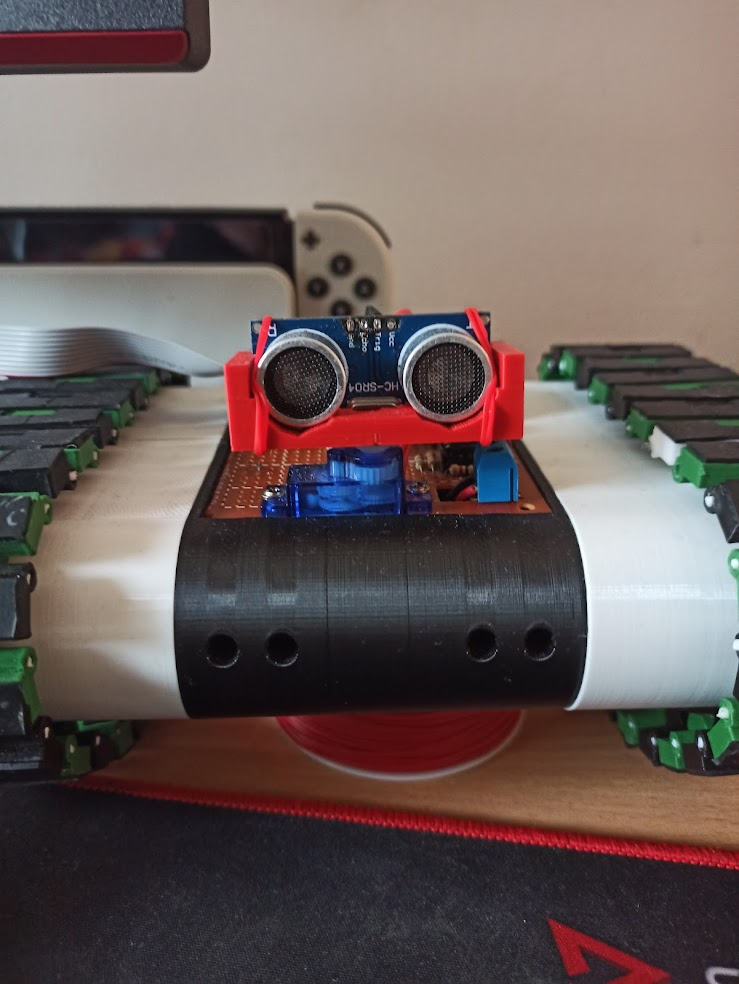
\includegraphics[height = 0.4\textheight]{Img/Azor.jpg}
        \caption{Zdjęcie „Azora”}
    \end{figure}

    \newpage
        \subsubsection{Schemat blokowy}
            \begin{figure}[!h]
    \centering
    \begin{circuitikz}
        \draw
            ( 0,  0) node [draw, rectangle, minimum width = 3cm, minimum height = 8cm](Atmega){ATmega}
            (-5,  1.75) node [draw, rectangle, minimum width = 3cm, minimum height = 2cm](HC_SR04){HC-SR04}
            (-5,  5) node [draw, rectangle, minimum width = 2cm, minimum height = 2cm](bt){HC05}
            ( 7,  1.5) node [draw, rectangle, minimum width = 2cm, minimum height = 2cm](com){QMC5883L}
            ( 7, -1.5) node [draw, rectangle, minimum width = 2cm, minimum height = 2cm](acc){MMA8451}
            ( 5,  4) node [draw, rectangle, minimum width = 2cm, minimum height = 1cm](eeprom){EEPROM}
            ( 5, -4) node [draw, rectangle, minimum width = 2cm, minimum height = 2cm](enkoder){Enkoder}
            
            (-5, -2) node [draw, rectangle, minimum width = 2cm, minimum height = 2cm](H_bridge){H Bridge}
            (-4, -5) node [draw, rectangle, minimum width = 2cm, minimum height = 2cm](servo){SG-90}
            (-7, -1.5) to[L] ++ (0, 1) -- ++ (1, 0) edge[bend left] ++ (0.5, -0.5)
            (-7, -1.5) -- ++ (1, 0)
            (-7, -3.5) to[L] ++ (0, 1) -- ++ (1, 0)
            (-7, -3.5) -- ++ (1, 0) edge[bend right] ++ (0.5, 0.5)

            % (3.25, -7) node [draw, rectangle, minimum width = 4cm, minimum height = 2cm, align=center, text width = 3cm](boostUp){Boost Up CN6009}
            % (-2.5, -7)node [draw, rectangle, minimum width = 2cm, minimum height = 2cm, text width = 2cm, align = center](BMS){Battery controller}
            % (0, -7.5) to[battery, invert] ++ (0, -1) node[ground]{}
            % (0, -7.5) -- ++ (-1.35, 0)
            % (0, -7.5) to[short, *-] ++ (1.3, 0)

            % (BMS) to[short, i=Enable] (boostUp)
            % (boostUp) ++(2, 0) -- ++(0.5, 0) -- ++ (0, 0.5) node[vcc]{$V_{CC}$}

            (eeprom) ++ (-0.5, -0.5) -- ++ (0, -5.5) -- ++ (1.4, 0)
            (eeprom) ++ ( 0,   -0.5) -- ++ (0, -5.0) -- ++ (0.9, 0)

            (com) ++ (-1.15, 0.5) to[short, -*] ++ (-0.85, 0) coordinate(sda)
            (com) ++ (-1.15, 0.0) to[short, -*] ++ (-1.35, 0) coordinate(scl)

            (sda) -- ++ (-1.5, 0) -- ++ (0, 1.5) coordinate(sda)
            (scl) -- ++ (-1.5, 0) -- ++ (0, 1.5) coordinate(scl)
            (sda) to[short] ++ (-2, 0)
            (scl) to[short] ++ (-1.5, 0)
            (sda) ++ (-1.25, 0) node[above]{SDA}
            (scl) ++ (-0.75, 0) node[below]{SCL}

            (sda) to[short, *-] ++ (0, 0.25) to[R] ++ (0, 2) node[vcc]{} ++ (-.25, 0.7) node[left]{$V_{CC}$}
            (scl) to[short, *-] ++ (0, 0.75) to[R] ++ (0, 2) node[vcc]{} ++ (0.25, 0.7) node[right]{$V_{CC}$}

            (bt) ++ (1, 0.25) to[short, i=RxD] ++ (2.00, 0) -- ++ (0, -1.75) -- ++ (0.50, 0)
            (bt) ++ (1,-0.25) to[short, i<_=TxD] ++ (1.75, 0) -- ++ (0, -1.75) -- ++ (0.75, 0)

            (HC_SR04) ++ (1.5, 0.25) to[short, i>=Echo] ++ (2.00, 0)
            (HC_SR04) ++ (1.5,-0.25) to[short, i<_=Trig] ++ (2.00, 0)

            (H_bridge) ++ (1, 0) to[short, i<=$\ $] ++ (1.5, 0) -- ++ (1, 0)

            (H_bridge) ++ (2.25, 0) node[above]{5}
            (H_bridge) ++ (2.25, 0) -- ++ ( 0.1,  0.1)
            (H_bridge) ++ (2.25, 0) -- ++ (-0.1, -0.1)

            (enkoder) ++ (-1, 0) -- ++ (-1, 0) -- ++ (0, 2) to[short, i>=$\ $] ++ (-1.5, 0)
            (servo) ++ (0.5, 1) -- ++ (0, 1) to[short, i<=$\ $] ++ (2, 0)
        ;
    \end{circuitikz}
    \caption{Schemat blokowy}
\end{figure}
    % \newpage
        
    \subsection{Środowisko programowe}
        \tab Program na ATmegę został napisany w języku C/C++, z wykorzystaniem bibliotek udostępnionych przez producenta.
        Do programowania, układu zostało wykorzystane narzędzie \textit{AVRdude} wraz z programatorem \textit{USBasp}.
        Natomiast graficzny interfejs dla komputerów klasy PC, został stworzony w Pythonie, z wykorzystaniem biblioteki ,,Turtle".


\end{document}